\documentclass{article}

\usepackage[a4paper]{geometry}
\usepackage[spanish]{babel}
\usepackage{xcolor}

\usepackage{mathbbol}
\usepackage{amsmath}
\usepackage{amsfonts}
\usepackage{hyperref}
\usepackage{graphicx}

% Cambiar 'Cuadro' -> 'Tabla'
\addto\captionsspanish{
    \renewcommand{\tablename}{Tabla}
}

\begin{document}

\begin{center}
    {\Large Aprendizaje Automático para Datos en Grafos} \\
    {\LARGE \textbf{Laboratorio 2}} \\
    \vspace{2em}
    \begin{minipage}{0.45\textwidth}
        \centering
        Graciana Castro \\
        4.808.848-2 \\
        gcastro@fing.edu.uy
    \end{minipage}
    \hfill
    \begin{minipage}{0.45\textwidth}
        \centering
        Julian O'Flaherty \\
        6.285.986-9 \\
        julian.o.flaherty@fing.edu.uy
    \end{minipage}
\end{center}


\section{Introducción}


Se presenta a continuación el informe del Laboratorio 2 para la materia Aprendizaje Automático para Datos en Grafos. El objetivo principal de este trabajo es analizar empíricamente propiedades estructurales de grandes redes reales y profundizar en el estudio de algoritmos de partición y detección de comunidades en grafos. A lo largo del laboratorio se busca validar conceptos teóricos vistos en clase, aplicando herramientas como \textit{NetworkX}, \textit{PyTorch Geometric} y \textit{graspologic}, y desarrollar habilidades para la interpretación de resultados obtenidos sobre diferentes tipos de grafos.

En la sección \ref{sec: datasets} del informe se presentan las bases de datos utilizadas en el laboratorio. En el primer ejercicio, presentado en la sección \ref{sec: estructuras}, se estudian propiedades globales y estructura de grandes redes, como la distribución de grados y la modularidad. Se trabaja con las bases de datos de citaciones entre papers y de vuelos entre aeropuertos. En la sección \ref{sec: comunidades} se implementan y comparan algoritmos espectrales para la partición y detección de comunidades en grafos, aplicándolos sobre el grafo de Zachary's Karate Club y sobre un grafo real de blogs políticos.

El código implementado puede consultarse en el repositorio de GitHub \url{https://github.com/j-oflaherty/AA-grafos/blob/main/lab2/Lab2_AAG2025.ipynb}.

\section{Bases de datos utilizadas} \label{sec: datasets}
Para este trabajo se utilizan las siguientes bases de datos:
\begin{itemize}
    \item \textbf{Citations (Cora)}: Esta base de datos contiene información sobre citaciones entre artículos científicos. Cada nodo representa un artículo, y una arista dirigida del nodo A al nodo B indica que el artículo A cita al artículo B. Es un grafo no dirigido que contiene 2708 nodos y 10556 aristas.
    \item \textbf{Airports}: Esta base de datos contiene información sobre vuelos entre aeropuertos. Cada nodo representa un aeropuerto, y una arista dirigida del nodo A al nodo B indica que existe un vuelo directo desde el aeropuerto A al aeropuerto B. Es un grafo dirigido que contiene 1190 nodos y 13599 aristas.
    \item \textbf{Zachary's Karate Club}: Presentada en el laboratorio anterior, esta base de datos representa las interacciones sociales entre los miembros de un club de karate. Cada nodo representa a un miembro del club, y una arista entre dos nodos indica que esos miembros interactúan socialmente.
    \item \textbf{Political Blogs}: Esta base de datos contiene información sobre blogs políticos y las conexiones entre ellos. Cada nodo representa un blog, y una arista entre dos nodos indica que el blog del que sale la arista tiene un link al blog al que llega la arista. Para el laboratorio se trabajará con la versión no dirigida, que tiene una arista entre dos nodos si existe una arista en cualquiera de los sentidos. Este grafo tiene 1490 nodos y 19025 aristas.
\end{itemize}


\section{Estructuras de grandes redes} \label{sec: estructuras}

\subsection{Distribución de grados}

La distribución de grados de un grafo $G$ se refiere al conjunto de fracciones $p_k$ que representan la proporción de vértices con grado $k$ en el grafo. Es una medida importante para caracterizar la estructura de la red, ya que proporciona información sobre cómo se conectan los nodos entre sí.


En muchas redes reales, como las redes sociales o las redes de citas académicas, la distribución de grados sigue una \textit{power-law}, que se define de la forma: $p_k = Ck^{-\alpha}$, donde $C$ es una constante de normalización y $\alpha$ es el exponente que caracteriza la distribución. Esta forma implica que la probabilidad de encontrar un nodo con grado $k$ disminuye rápidamente a medida que $k$ aumenta.


En la figura \ref{fig: degree_distribution} se muestra la distribución de grados del grafo de citaciones entre papers. Se observa que existe un rango de $k$ para el cual la distribución sigue una \textit{power-law}; sin embargo, no se cumple para todos los valores (hecho que no resulta extraño en redes reales). Para evidenciar si efectivamente la distribución sigue una \textit{power-law} en cierto rango, se realiza la gráfica utilizando \textit{bins} equiespaciados, donde la tendencia lineal se hace más evidente.

\begin{figure}
    \centering
    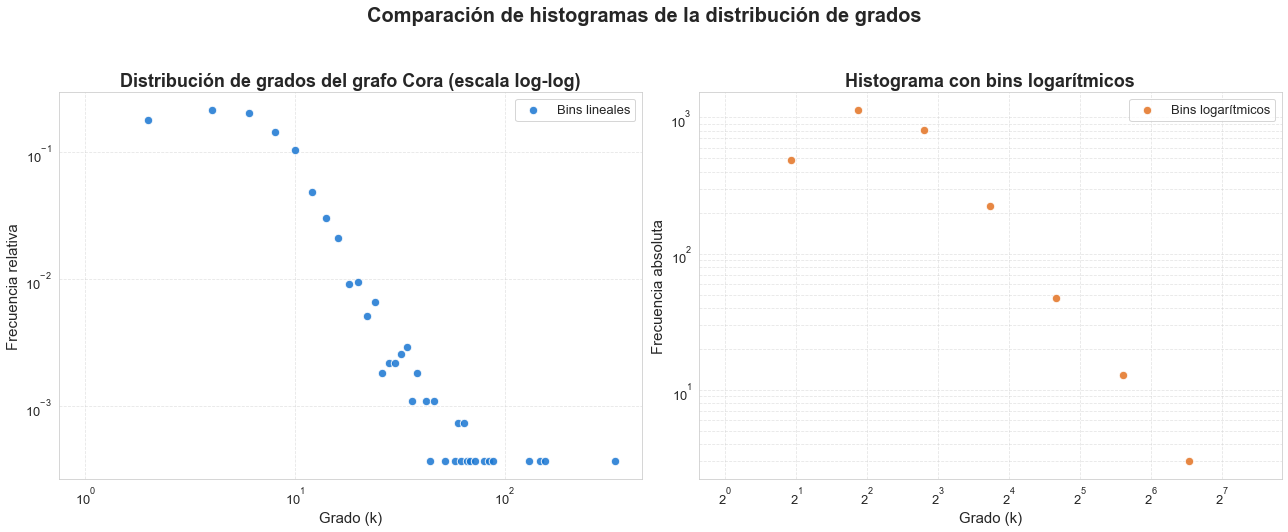
\includegraphics[width=0.8\textwidth]{imagenes/dist_grado_Cora.png}
    \caption{Distribución de grados del grafo de citaciones entre papers. En la figura (a) se observa la distribución en escala logarítimica, mientras que en la figura (b) se muestra en bins equiespaciados.}
    \label{fig: degree_distribution}
\end{figure}


La distribución que se observa en la figura \ref{fig: degree_distribution}(b) sigue la denominada \textit{Distribución de Pareto}. Una variable aleatoria $X$ se dice que tiene distribución de Pareto si tiene una función de densidad de probabilidad dada por:

$$p(k) = \left\lbrace \begin{array}{c c} C k^{-\alpha} & \text{ si } k\geq k_\text{min} \\ 0 & \text{ en otro caso} \end{array}\right.$$


Para hallar el $C$ que verifica que esta distribución es una densidad, se integra sobre su dominio y se iguala a 1:

$$
    \int_{0}^{\infty} p(k) dk = \int_{k_{\text{min}}}^{\infty} C k^{-\alpha} dk = C \int_{k_{\text{min}}}^{\infty} k^{-\alpha}dk \\
    \int_{0}^{\infty} p(k) dk = C \left[ \frac{k_{\text{min}}^{-\alpha+1}}{-\alpha+1} \right] = 1 \\
    \Rightarrow C = \frac{-\alpha+1}{k_{\text{min}}^{-\alpha+1}}
$$


Como se demuestra en la sección \ref{sec: pareto}, el estimador de máxima verosimilitud para el exponente $\alpha$ de la distribución de Pareto es:

$$
    \hat{\alpha} = 1 + n \left[ \sum_{i=1}^{n} \ln\left(\frac{k_i}{k_{\text{min}}}\right) \right]^{-1}.
$$


Para calcularlo, se implementa una función que recibe como parámetros una lista de los grados de un grafo y el valor de $k$ a partir del cual vale la \textit{power-law}. Aplicando esta función al grafo de citaciones entre papers, considerando $k_{\text{min}} = 10$, se obtiene un valor de $\hat{\alpha} = 4.030$.

\subsection{Assortative Mixing}

Se define el \textit{assortative mixing} como la tendencia de los nodos en una red a conectarse con otros nodos que son similares en algún aspecto. En el contexto de redes sociales, por ejemplo, esto puede significar que las personas tienden a formar conexiones con otras personas que tienen intereses, antecedentes o características demográficas similares. Se utiliza como medida de similaridad la \textit{modularidad}, que mide la proporción entre las aristas que hay entre nodos de un mismo tipo y las esperadas si la asignación de aristas fuera aleatoria. Formalmente, está definida como:

$$Q = \frac{1}{2m} \sum_{ij} \left(A_{ij} -\frac{k_ik_j}{2m} \right)\delta(c_i,c_j)$$

donde $m$ es la cantidad total de aristas en la red, $A_{ij}$ son las entradas de la matriz de adyacencia, $k_i$ es el grado del nodo $i$ y $\delta(r,p)$ es la delta de Kronecker: $\delta(r,p) = 1$ si $r=p$ y $\delta(r,p) = 0$ si $r\neq p$. Toma valores mayores a uno si hay mucha interconexión entre nodos del mismo tipo, y valores menores a uno en el caso contrario.


Para el cálculo de modularidad, se utiliza primero una función que recibe las etiquetas del grafo para separarlo en comunidades y luego calcula la modularidad utilizando la función \verb|networkx.algorithms.community.modularity|. Se obtienen los siguientes resultados para las bases de datos de citaciones entre papers y de vuelos entre aeropuertos:
\begin{itemize}
    \item \textbf{Citations (Cora)}: La modularidad obtenida es $Q = 0.640$.
    \item \textbf{Airports}: La modularidad obtenida es $Q = 0.108$.
\end{itemize}

Se entiende que es coherente que la modularidad del grafo de aeropuertos sea baja, ya que los aeropuertos poco transitados suelen tener vuelos hacia aeropuertos más grandes, y no entre ellos. La modularidad del grafo de citaciones es más alta, ya que los artículos tienden a citar otros artículos relacionados a la misma disciplina.

\section{Detección de comunidades} \label{sec: comunidades}

\section{Estimador de máxima verosimilitud para el exponente de la distribución de Pareto} \label{sec: pareto}

Sea $X$ una variable aleatoria con distribución de Pareto, por lo tanto su función de densidad de probabilidad es:

$$p(x) = \left\lbrace \begin{array}{c c} C x^{-\alpha} & \text{ si } x\geq x_\text{min} \\ 0 & \text{ en otro caso} \end{array}\right.$$

\subsection{Función de log-verosimilitud}

La función de log-verosimilitud para una muestra $x_1, x_2, \ldots, x_n$ es la suma de los logaritmos de las funciones de densidad evaluadas en cada punto de la muestra. Para el ejercicio presentado en la sección \ref{sec: estructuras}, en que se tiene una Distribución de Pareto con $C = \frac{-\alpha+1}{k_{\text{min}}^{-\alpha+1}}$, se halla la función de log-verosimilitud:

\begin{align}
    \mathcal{L}_n(\alpha) & = \log \left[\prod_{i=1}^{n} \left( \frac{1-\alpha}{k_{\text{min}}^{1-\alpha}} k_i^{-\alpha} \right) \right] \nonumber               \\
                          & = \sum_{i=1}^{n} \left[ \log(1-\alpha) - log\log(k_{\text{min}}) - \log \left(\frac{k_i}{k_{min}} \right)^{\alpha} \right] \nonumber \\
                          & = n \log(1-\alpha) - n\log(k_{\text{min}}) - \alpha \sum_{i=1}^{n} \log\left(\frac{k_i}{k_{min}} \right)
\end{align}

donde en la primera igualdad se toma el logaritmo, en la segunda se utiliza la propiedad de que el logaritmo del producto es la suma de los logaritmos, y en la tercera se resuelven las sumatorias que no dependen de $i$ y se utiliza la propiedad del logaritmo de la potencia.

\subsection{Estimador de Máxima Verosimilitud para $\alpha$}

Partiendo de la ecuación \ref{eq: log-verosimilitud}, se deriva respecto a $\alpha$ e iguala a cero para encontrar el máximo:
$$
    \frac{d\mathcal{L}_n(\alpha)}{d\alpha} = \frac{n}{\alpha -1} - \sum_{i=1}^n \log \left(\frac{k_i}{k_\text{min}}\right) = 0 \\
    \Rightarrow \frac{n}{\alpha -1} = \sum_{i=1}^n \log \left(\frac{k_i}{k_\text{min}}\right) \\
    \Rightarrow \hat{\alpha} = 1 + n \left[ \sum_{i=1}^{n} \ln\left(\frac{k_i}{k_\text{min}}\right) \right]^{-1}
$$



\end{document}